\documentclass[12pt]{extarticle}

\usepackage{amsmath}
\usepackage{unicode-math}
\usepackage{xltxtra}
\usepackage{xgreek}

\setmainfont{Liberation Serif}

\usepackage{tabularx}

\pagestyle{empty}

\usepackage{geometry}
\geometry{a4paper, total={190mm,275mm}, left=10mm, top=10mm}

\usepackage{graphicx}
\graphicspath{ {images/} }

\usepackage{wrapfig}

\begin{document}
\renewcommand{\labelenumi}{\alph{enumi})}
\renewcommand{\labelenumii}{\roman{enumii}.}

\begin{table}
    \small
    \begin{tabularx}{\textwidth}{ c X r }
        \begin{tabular}{ c }
            
\includegraphics[scale=0.4]{ελληνική}         \\
            ΕΛΛΗΝΙΚΗ ΔΗΜΟΚΡΑΤΙΑ                           \\
            ΥΠΟΥΡΓΕΙΟ ΠΑΙΔΕΙΑΣ \& ΘΡΗΣΚΕΥΜΑΤΩΝ            \\
            ΠΕΡΙΦΕΡΕΙΑΚΗ Δ/ΝΣΗ Α/ΘΜΙΑΣ \& Β/ΘΜΙΑΣ ΕΚΠ/ΣΗΣ \\
            ΚΕΝΤΡΙΚΗΣ ΜΑΚΕΔΟΝΙΑΣ                          \\
            Δ/ΝΣΗ Β/ΘΜΙΑΣ ΕΚΠ/ΣΗΣ ΑΝ. ΘΕΣ/ΝΙΚΗΣ           \\
            10ο ΓΕΝΙΚΟ ΛΥΚΕΙΟ ΘΕΣ/ΝΙΚΗΣ
        \end{tabular}
         &  &
        \begin{tabular}{ r }
            Σχολικό Έτος: 2022 - 2023               \\
            Εξ. Περίοδος: Μαΐου - Ιουνίου           \\
            Μάθημα: Γεωμετρία Α Λυκείου             \\
            Εισηγητές: Γιαννόπουλος, Κράντας, Λόλας \\ \\
            Θεσσαλονίκη, 09 / 06 / 2023
        \end{tabular}
    \end{tabularx}
\end{table}

\part*{\centering{Θέματα}}
\section*{Θέμα 1}
\noindent

\begin{enumerate}
    \item[α)] Να αποδείξετε ότι το άθροισμα των γωνιών κάθε τριγώνου είναι 2 ορθές. \hspace*{\fill} \textbf{Μονάδες 15}

    \item[β)] Να χαρακτηρίσετε τις παρακάτω προτάσεις με Σωστό ή Λάθος
        \begin{enumerate}
            \item Δύο τρίγωνα που έχουν τις τρεις γωνίες τους ίσες, μία προς μία, τότε είναι ίσα
            \item Το τμήμα που συνδέει τα μέσα δύο πλευρών ενός τριγώνου είναι παράλληλο στη τρίτη πλευρά και ίσο με το μισό της
            \item Σε κάθε ορθογώνιο τρίγωνο αν η μία γωνία του είναι $30^{\circ}$ τότε η απέναντι κάθετη πλευρά ισούται με το μισό της υποτείνουσας
            \item Η διάμεσος σε ένα ισοσκελές τρίγωνο είναι και ύψος
            \item Οι διαγώνιοι του παραλληλογράμμου τέμνονται κάθετα\hspace*{\fill}\textbf{Μονάδες 10}
        \end{enumerate}
\end{enumerate}

\section*{Θέμα 2 (13653)}
\noindent
Σχεδιάζουμε γωνία $x\hat{O}y=60^{\circ}$ και παίρνουμε σημείο $Α$ επί της πλευράς $Ox$, τέτοιο ώστε $ΑΟ=2$. Φλερουμε τη διχοτόμο $Οδ$ της γωνίας $x\hat{O}y$ και θεωρούμε σημείο $Μ$ στην $Οδ$, ώστε $ΑΜ=ΑΟ$. Να υπολογίσετε:
\begin{figure}[h]
    \centering
    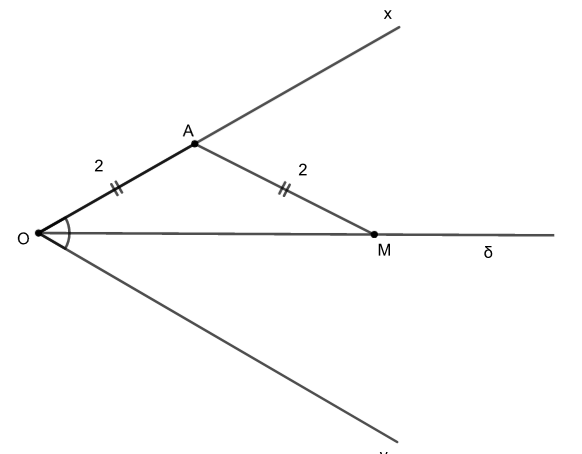
\includegraphics[width=0.50\textwidth]{2023_2}
\end{figure}
\begin{enumerate}
    \item[α)] Τη γωνία $δ\hat{Ο}y$. \hspace*{\fill} \textbf{Μονάδες 6}
    \item[β)] Τις γωνίες του τριγώνου $ΑΟΜ$ \hspace*{\fill} \textbf{Μονάδες 9}
    \item[γ)] Το μήκος του ύψους $ΑΒ$ που αντιστοιχεί στη βάση $ΟΜ$ του ισοσκελούς τριγώνου $ΑΟΜ$ \hspace*{\fill} \textbf{Μονάδες 10}
\end{enumerate}


\section*{Θέμα 3}
\noindent

\begin{wrapfigure}[3]{r}{0.38\textwidth}
    \centering
    \vspace{-60pt}
    % \hspace{-80pt}
    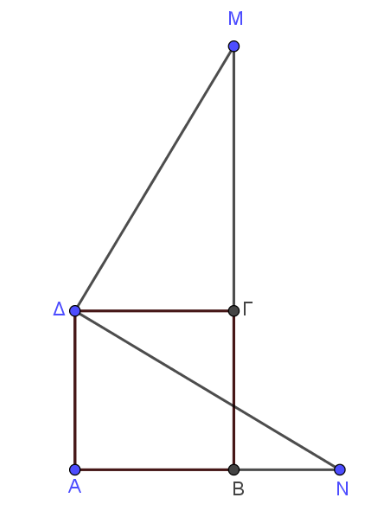
\includegraphics[width=0.25\textwidth]{2023_3}
\end{wrapfigure}



\noindent
Στο τετράγωνο $ΑΒΓΔ$ προεκτείνουμε την πλευρά $ΑΒ$ κατά τμήμα $ΒΝ$ και την πλευρά $ΒΓ$ κατά τμήμα $ΓΜ=ΑΝ$. Να αποδείξετε ότι
\begin{enumerate}
    \item[α)] $ΔΝ=ΔΜ$ \hspace*{\fill} \textbf{Μονάδες 12}
    \item[β)] $ΔΝ\perp ΔΜ$ \hspace*{\fill} \textbf{Μονάδες 13}
\end{enumerate}


\hfill \break
\section*{Θέμα 4 (1824)}
\noindent

Δίνεται τρίγωνο $ΑΒΓ$ και στην προέκταση της $ΓΒ$ (προς το $Β$) θεωρούμε σημείο $Δ$ τέτοιο ώστε $ΒΔ=ΑΒ$ ενώ στην προέκταση της $ΒΓ$ (προς το $Γ$) θεωρούμε σημείο $Ε$ τέτοιο ώστε $ΓΕ=ΓΑ$.

Αν οι εξωτερικοί διχοτόμοι των γωνιών $Β$ και $Γ$ τέμνουν τις $ΑΔ$ και $ΑΕ$ στα σημεία $Κ$ και $Λ$ αντίστοιχα και η $ΚΛ$ τέμνει τις $ΑΒ$ και $ΑΓ$ στα σημεία $Μ$ και $Ν$ αντίστοιχα, να αποδείξετε ότι:
\begin{enumerate}
    \item[α)] Τα σημεία $Κ$ και $Λ$ είναι μέσα των $ΑΔ$ και $ΑΕ$ αντίστοιχα \hspace*{\fill} \textbf{Μονάδες 8}

    \item[β)] Τα τρίγωνα $ΚΜΑ$ και $ΑΝΛ$ είναι ισοσκελή. \hspace*{\fill} \textbf{Μονάδες 9}
    \item[γ)] $ΚΛ=\dfrac{ΑΒ+ΑΓ+ΒΓ}{2}$ \hspace*{\fill} \textbf{Μονάδες 8}
\end{enumerate}
\begin{figure}[h]

    \centering
    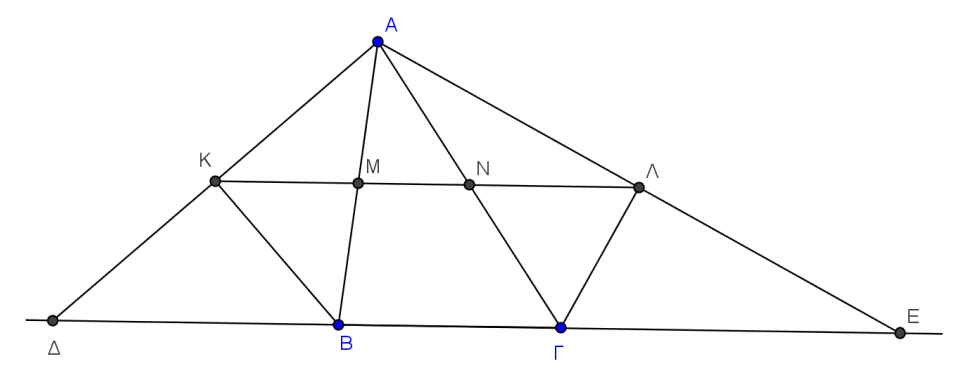
\includegraphics[width=0.80\textwidth]{2023_4}
\end{figure}

\begin{table}[htb]
    \begin{tabularx}{\textwidth}{ X c X c X}
         &
        \begin{tabular}[t]{ c }
            Ο Δ/ντης \\ \\ \\ \\
            Παπαδημητρίου Χρήστος
        \end{tabular}
         &   &
        \begin{tabular}[t]{ c }
            Ο εισηγητές           \\ \\ \\ \\
            Γιαννόπουλος Σωτήριος \\ \\ \\ \\
            Κράντας Στυλιανός     \\ \\ \\ \\
            Λόλας Κωνσταντίνος    \\ \\
        \end{tabular}
         &
    \end{tabularx}
\end{table}
\end{document}